% --------------------------------------------------------------
% This is all preamble stuff that you don't have to worry about.
% Head down to where it says "Start here"
% --------------------------------------------------------------
 
\documentclass[12pt]{article}
 
\usepackage[margin=1in]{geometry} 
\usepackage{amsmath,amsthm,amssymb, mathtools}
\usepackage{hyperref}
\usepackage{graphicx}
\usepackage{float}
\graphicspath{./data/}



\newcommand{\N}{\mathbb{N}}
\newcommand{\Z}{\mathbb{Z}}

\newtheorem*{remark}{Remark}
 
\newenvironment{theorem}[2][Theorem]{\begin{trivlist}
\item[\hskip \labelsep {\bfseries #1}\hskip \labelsep {\bfseries #2.}]}{\end{trivlist}}
\newenvironment{lemma}[2][Lemma]{\begin{trivlist}
\item[\hskip \labelsep {\bfseries #1}\hskip \labelsep {\bfseries #2.}]}{\end{trivlist}}
\newenvironment{exercise}[2][Exercise]{\begin{trivlist}
\item[\hskip \labelsep {\bfseries #1}\hskip \labelsep {\bfseries #2.}]}{\end{trivlist}}
\newenvironment{problem}[2][Problem]{\begin{trivlist}
\item[\hskip \labelsep {\bfseries #1}\hskip \labelsep {\bfseries #2.}]}{\end{trivlist}}
\newenvironment{question}[2][Question]{\begin{trivlist}
\item[\hskip \labelsep {\bfseries #1}\hskip \labelsep {\bfseries #2.}]}{\end{trivlist}}
\newenvironment{corollary}[2][Corollary]{\begin{trivlist}
\item[\hskip \labelsep {\bfseries #1}\hskip \labelsep {\bfseries #2.}]}{\end{trivlist}}

\newenvironment{solution}{\begin{proof}[Solution]}{\end{proof}}
 

\begin{document}

 
% --------------------------------------------------------------
%                         Start here
% --------------------------------------------------------------
 
\title{Project \\ Low-Rank Matrix Completion}
\author{Alireza Naderi, 
Milad Jalali}

\maketitle

\section{Background}
The Frank-Wolfe algorithm, also known as Conditional Gradient Method, is an iterative first-order algorithm for solving constrained convex optimization problems that has long been in use \cite{FW}. In each step, it minimizes a linear approximation of the convex function $f(\cdot)$ over the compact convex domain $\mathcal{D}$, and then determines $\mathbf{x}^{(k+1)}$ on the line segment between $\mathbf{x}^{(k)}$ and the linear minimizer $\mathbf{s}^{(k)}$, i.e.
\begin{equation}
    \mathbf{x}^{(k+1)} = \mathbf{x}^{(k)} + \gamma_k (\mathbf{s}^{(k)} - \mathbf{x}^{(k)}),
\end{equation}
where $\gamma_k \in [0,1]$ is the \textit{step size} and $\mathbf{s}^{(k)} \in \mathrm{argmin}_{\mathbf{s} \in \mathcal{D}} \langle \nabla f(\mathbf{x}^{(k-1)}), \mathbf{s} \rangle$. It has been known that the choice $\gamma_k = \frac{2}{k+2}, \, k=0,1,2,...$ guarantees the convergence of the algorithm with rate $O(1/k)$, i.e. $f(\mathbf{x}^{(k)}) - f(\mathbf{x}^*) \leq O(1/k)$, where $\mathbf{x}^*$ is an optimal solution \cite{DH}.

There are some variants of the algorithm proposed in the literature that improve upon the vanilla version in the following ways:
\begin{itemize}
    \item Approximate linear subproblems: Instead of finding the exact minimizer $\mathbf{s}^{(k)}$ in each step, this variant uses an approximation $\mathbf{\Tilde{s}}^{(k)}$ such that
    \begin{equation}\label{eq2}
        \langle \nabla f(\mathbf{x}^{(k-1)}), \mathbf{\Tilde{s}}^{(k)} \rangle \leq \langle \nabla f(\mathbf{x}^{(k-1)}), \mathbf{{s}}^{(k)} \rangle + \frac{1}{2} \delta C_f.
    \end{equation}
    Here,
    \begin{equation}
        C_f \coloneqq \max_{\substack{\mathbf{x},\mathbf{s} \in \mathcal{D} \\ \gamma \in [0,1] \\ \mathbf{y} = \mathbf{x} + \gamma (\mathbf{s} - \mathbf{x})}} \frac{2}{\gamma^2} \big( f(\mathbf{y}) - f(\mathbf{x}) - \langle \mathbf{y}-\mathbf{x}, \nabla f(\mathbf{x}) \rangle \big)
    \end{equation}
    is called the \textit{curvature constant} of $f$.
    \item Optimizing the line search: Instead of using fixed step sizes $\gamma_k = \frac{2}{k+2}$, this variant attempts to find the best step size in each iteration by setting
    \begin{equation}
        \gamma_k = \mathrm{argmin}_{\gamma \in [0,1]} \; f \big( \mathbf{x}^{(k)} + \gamma (\mathbf{s}^{(k)} - \mathbf{x}^{(k)}) \big).
    \end{equation}
    
    \item Fully corrective updates: Instead of restricting $\mathbf{x}^{(k+1)}$ to lie on the line segment between $\mathbf{x}^{(k)}$ and $\mathbf{s}^{(k)}$, this variant uses the information from all the previous iterations, searching for a minimizer on the convex hull $\mathcal{C} \coloneqq \mathrm{conv} \{\mathbf{x}^{(0)}, \mathbf{s}^{(1)},...,\mathbf{s}^{(k)}\}$, i.e.
    \begin{equation}
        \mathbf{x}^{(k+1)} = \mathrm{argmin}_{\mathbf{x} \in \mathcal{C}} \; f(\mathbf{x}). 
    \end{equation}
\end{itemize}

\section{Theory}

In his paper \cite{J}, Jaggi proves the convergence in \textit{primal error} as well as in \textit{duality gap} for all the abovementioned variants of the Frank-Wolfe algorithm. Besides, he shows that the algorithm is also robust to inaccurate gradient information, and the convergence analysis is invariant under arbitrary affine transformation of the domain. We briefly mention the main results here.
\begin{theorem}{1}
The following holds for all the above variants of the Frank-Wolfe algorithm:
\begin{equation}
    f(\mathbf{x}^{(k)}) - f(\mathbf{x}^{*}) \leq \frac{2C_f}{k+2}(1+\delta), \quad \forall k \geq 1,
\end{equation}
where $\delta$ is the level of accuracy in solving linear subproblems as in expression (\ref{eq2}) and $C_f$ is the curvature constant of $f$.
\end{theorem}

Now we turn to the \textit{primal-dual convergence}. The quantity $g(\mathbf{x}) \coloneqq \max_{\mathbf{s} \in \mathcal{D}} \langle \mathbf{x}-\mathbf{s}, \nabla f(\mathbf{x}) \rangle$ can be shown to be the actual \textit{duality gap} for the primal problem. Using indicator function $I_{\mathcal{D}}$, we can rewrite the original problem as
\begin{equation}
    \min_{\mathbf{x}} \: f(\mathbf{x}) + I_{\mathcal{D}}(\mathbf{x}).
\end{equation}
Hence, the dual problem would be
\begin{equation}
    \max_{\mathbf{u}} \: -f^{*}(\mathbf{u}) - \sigma_{\mathcal{D}}(-\mathbf{u}),
\end{equation}
where $\sigma_{\mathcal{D}}(\cdot) \coloneqq \sup_{\mathbf{d}\in \mathcal{D}} \langle \cdot, \mathbf{d} \rangle$ is the support function of $\mathcal{D}$ and $f^{*}(\mathbf{u}) \coloneqq \sup_{\mathbf{x}} \big( \langle \mathbf{u},\mathbf{x} \rangle -f(\mathbf{x})\big)$ is the Fenchel conjugate of $f$ (see \cite{B} for more on duality). Therefore, the duality gap at $(\mathbf{x},\mathbf{u})$ is
\begin{equation}
    h(\mathbf{x},\mathbf{u}) \coloneqq f(\mathbf{x})+I_{\mathcal{D}}(\mathbf{x}) + f^{*}(\mathbf{u}) + \sigma_{\mathcal{D}}(-\mathbf{u}).
\end{equation}
Using Fenchel's equality and evaluating the gap at $(\mathbf{x},\mathbf{u}) = (\mathbf{x}^{(k)}, \nabla f(\mathbf{x}^{(k)}))$, we get
\begin{equation}
    h(\mathbf{x},\mathbf{u}) = \langle \mathbf{x}^{(k)},\nabla f(\mathbf{x}^{(k)}) \rangle + \sup_{\mathbf{s} \in \mathcal{D}} \langle \mathbf{s}, -\nabla f(\mathbf{x}^{(k)}) \rangle = g(\mathbf{x}^{(k)}). 
\end{equation}
Furthermore, convexity of $f$ readily implies
\begin{equation}
    f(\mathbf{x}) - f(\mathbf{x}^{*}) \leq g(\mathbf{x}),
\end{equation}
i.e. the duality gap is a certificate for the approximation quality. The following theorem guarantees the convergence of the duality gap.
\begin{theorem}{2}
If any of the abovementioned variants of the Frank-Wolfe algorithm is run for $K\geq 2$ iterations, then there exists $1 \leq \hat{k} \leq K$ such that
\begin{equation}
    g(\mathbf{x}^{(\hat{k})}) \leq \frac{27 C_f}{4(K+2)} (1+\delta).
\end{equation}
\end{theorem}

\section{Application}
The output of a Frank-Wolfe-type algorithm, by construction, lies in the convex hull of a few so-called "atoms". Thus, the solution has a natural atomic decomposition, where the set of atoms consists of the extreme points of $\mathcal{D}$. Interestingly, a broad range of existing methods for optimization over the convex hull of an atomic set (e.g. sparse vectors or low-rank matrices) can be unified under this approach.

Besides, for many choices of the domain, the linear subproblems that occur in each iteration of the Frank-Wolfe algorithm can be solved more efficiently than a general LP. Of particular importance is the norm-regularized problem
\begin{equation}
    \min f(\mathbf{x}) \quad \mathrm{s.t.} \: \: ||\mathbf{x}|| \leq \tau,
\end{equation}
where $||\cdot||$ is some (vector or matrix) norm, i.e. $\mathcal{D} = \tau \mathbb{B}_{||\cdot||}$.

As an example, consider the case $\mathcal{D} = \mathbb{B}_p$. It is straightforward to show (e.g. see \cite{T})
\begin{equation}
    \mathbf{s}^{(k)}_i = -\alpha \cdot \mathrm{sign}\big(\nabla f_i(\mathbf{x}^{(k-1)})\big) \cdot \big|\nabla f_i(\mathbf{x}^{(k-1)}) \big|^{p-1},
\end{equation}
where $\alpha$ is chosen so that $||\mathbf{s}^{(k)}||_p = 1$. Since an analytical solution exists for each coordinate, the linear minimization subproblem can be solved in linear time.

Another problem that illustrates the computational advantage of the Conditional Gradient Method over the Projected Gradient Method is the trace-regularized problem,
\begin{equation}
    \min f(X) \quad \mathrm{s.t.} \: \: ||X||_{\mathrm{tr}} \coloneqq \sum_{i} |\sigma_i(X)| \leq 1.
\end{equation}
It can be shown that the minimizer of the internal subproblem is $S^{(k)} = - \mathbf{u}\mathbf{v}^\top$, where $\mathbf{u}$ and $\mathbf{v}$ are (respectively) the leading left and right singular vectors of $\nabla f(X^{(k)})$. Thus, one only needs to compute (or approximate) the leading singular vectors, while the complete SVD is necessary to perform the Projected Gradient Method. A list of some other optimization domains and their respective computational complexities can be found in Table 1 of \cite{J}.

\section{Low-Rank Matrix Completion: Factored Updates}

\section{Dual Version with Primal Recovery}
In Fan et al. \cite{FJSF}, the authors propose a dual version of the Frank-Wolfe method (aka Conditional Gradient) for the constrained least-squares problem
\begin{equation*}
    \min_{\mathbf{x} \in \hat{\mathcal{A}}} \frac{1}{2} ||M\mathbf{x} - \mathbf{b}||_2^2.
\end{equation*}
The algorithm 6.3, instead of tracking the primal iterates $\mathbf{x}^{(k)}$, attempts to find the optimal negative gradient $\mathbf{z}^{*} = - \nabla f(\mathbf{x}^{*})$ through iterations $\mathbf{z}^{(k)} \rightarrow \mathbf{z}^{*}$. In each iteration, the intermediate vectors are to satisfy

    \begin{align*}
        \mathbf{r}^{(k)} &= \mathbf{b} - M \mathbf{x}^{(k)}, \\
        \mathbf{z}^{(k)} &= M^* \mathbf{r}^{(k)}, \\
        \mathbf{p}^{(k)} &= M\mathbf{a}^{(k)}, \quad \quad \mathbf{a}^{(k)} \in \mathcal{F}_{\mathcal{A}}(\mathbf{z}^{(k)}), \\
        \mathbf{q}^{(k)} &= M\mathbf{x}^{(k)}, \\
        \Delta \mathbf{r}^{(k)} &= \mathbf{p}^{(k)} - \mathbf{q}^{(k)}.
    \end{align*}

When the desired optimality condition is met after $K$ iterations, one finds the primal optimal solution as
\begin{equation*}
    \mathbf{x}^{(K)} \in \mathrm{argmin}_{\mathbf{x}} \{||M\mathbf{x} - \mathbf{b}||_2^2 \; | \; \mathcal{S}_{\mathcal{A}}(\mathbf{x}) \subseteq \tau \mathcal{E}_{\mathcal{A}}(\mathbf{z}^{(K)})\}.
\end{equation*}

A useful special case is the problem of low-rank matrix completion, where the "low-rank"ness is encouraged by constraining the nuclear norm:
\begin{equation*}
    \min_{X \in \mathbb{R}^{m \times n}} \frac{1}{2} ||\Omega \circ X - B||_{F}^2 \quad \mathrm{s.t.} \: ||X||_{*} \leq \tau.
\end{equation*}
The problems most prevalently arises in recommender systems, where the zero-one mask $\Omega$ encodes whether or not the user $i$ has rated the product $j$. The algorithm 6.4 of \cite{FJSF} specializes the more general algorithm 6.3 for the low-rank matrix estimation problem.

As suggested by the writers for the implementation, we have generated the "true" underlying matrix to be the addition of a low-rank one and a gaussian "noise":
\begin{equation*}
    B = UV^\top + 0.1 \cdot N,
\end{equation*}
where $U \in \mathbb{R}^{m \times r}$, $V \in \mathbb{R}^{n \times r}$, and $N \in \mathbb{R}^{m \times n}$ are i.i.d. standard gaussian matrices. The rank $r$ is set to $\frac{m}{100}$ and the mask $\Omega$'s entries are $\mathrm{Bernoulli}(p)$ random variables. Other parameters to set are the threshold $\epsilon$ used in the optimality check, and $\ell$, the number of singular vectors to keep from the singular value decomposition of $Z^{(k)}$. In the below results $\ell = 5r$, $\tau = r$, $m = n$, and the parameters $p$ and $\epsilon$ take different values. The following plots show the error, the elapsed time, and the so-called "effective rank" of the primal solution, which is simply the number of singular values that account for the 90\% of the total Frobenius norm.

\begin{figure}[H]
    \centering
    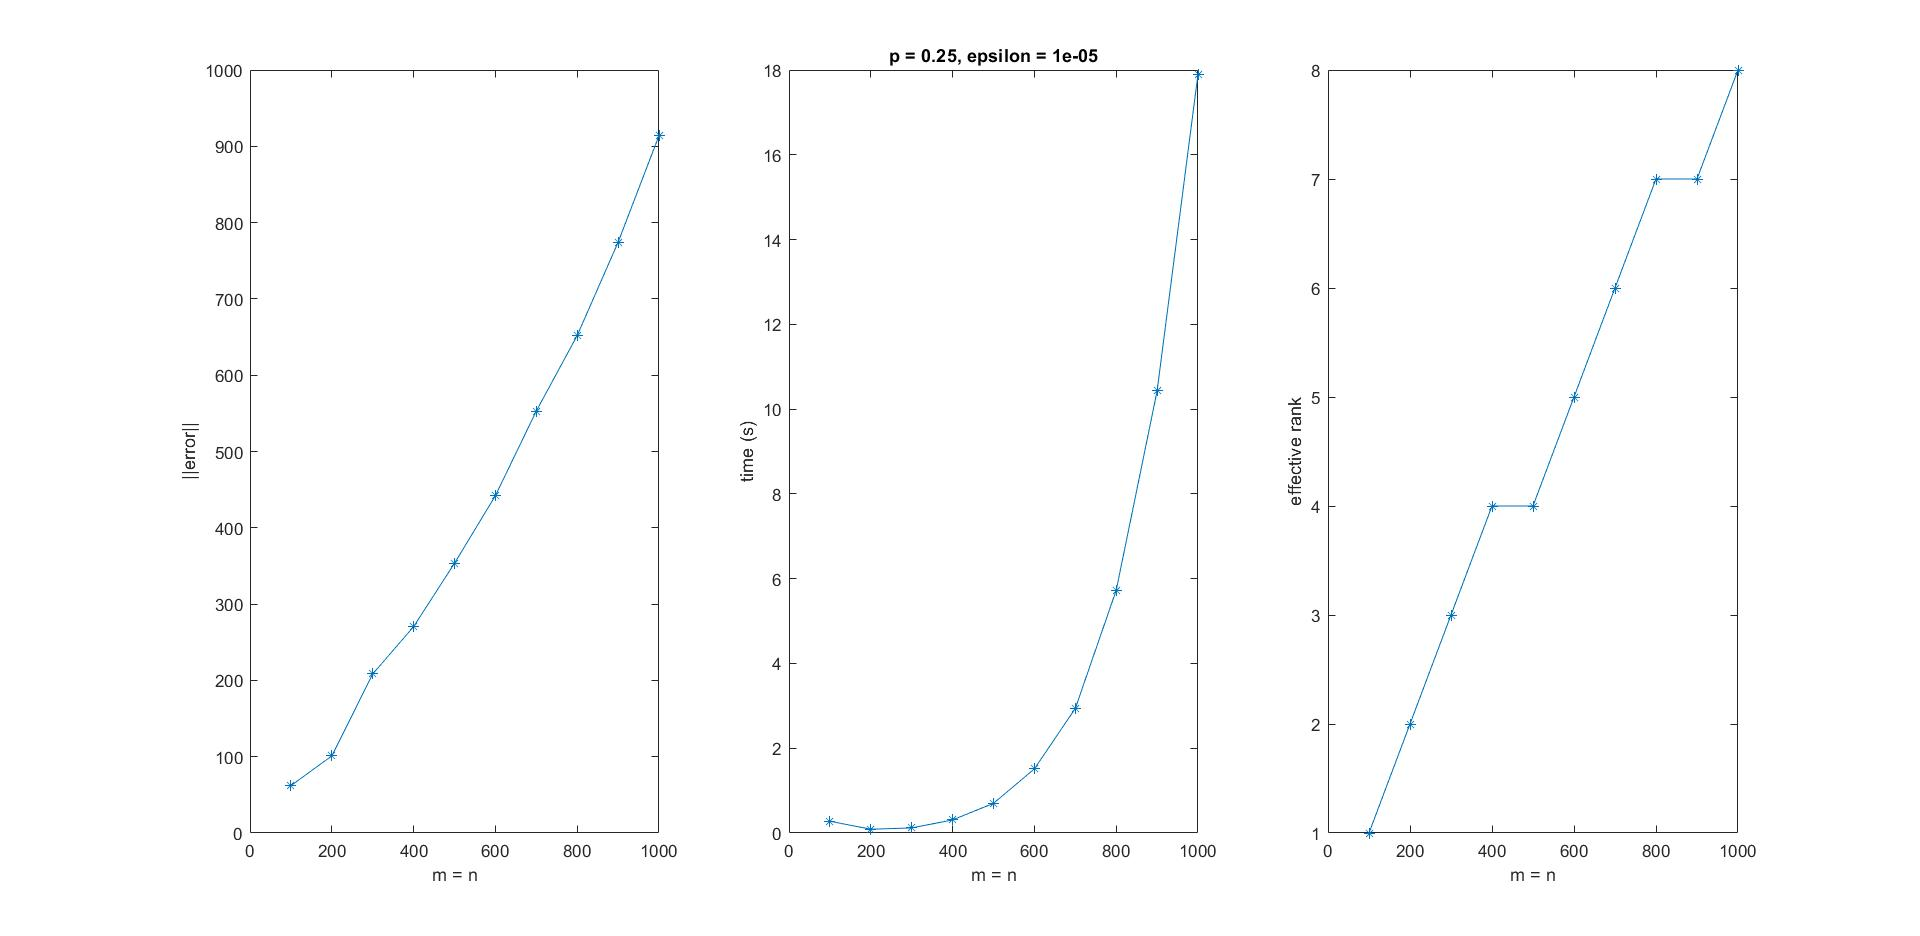
\includegraphics[width=\textwidth]{data/p4.jpg}
    \caption{$p = 0.25$, $\epsilon = 10^{-5}$}
    \label{img1}
\end{figure}
\begin{figure}[H]
    \centering
    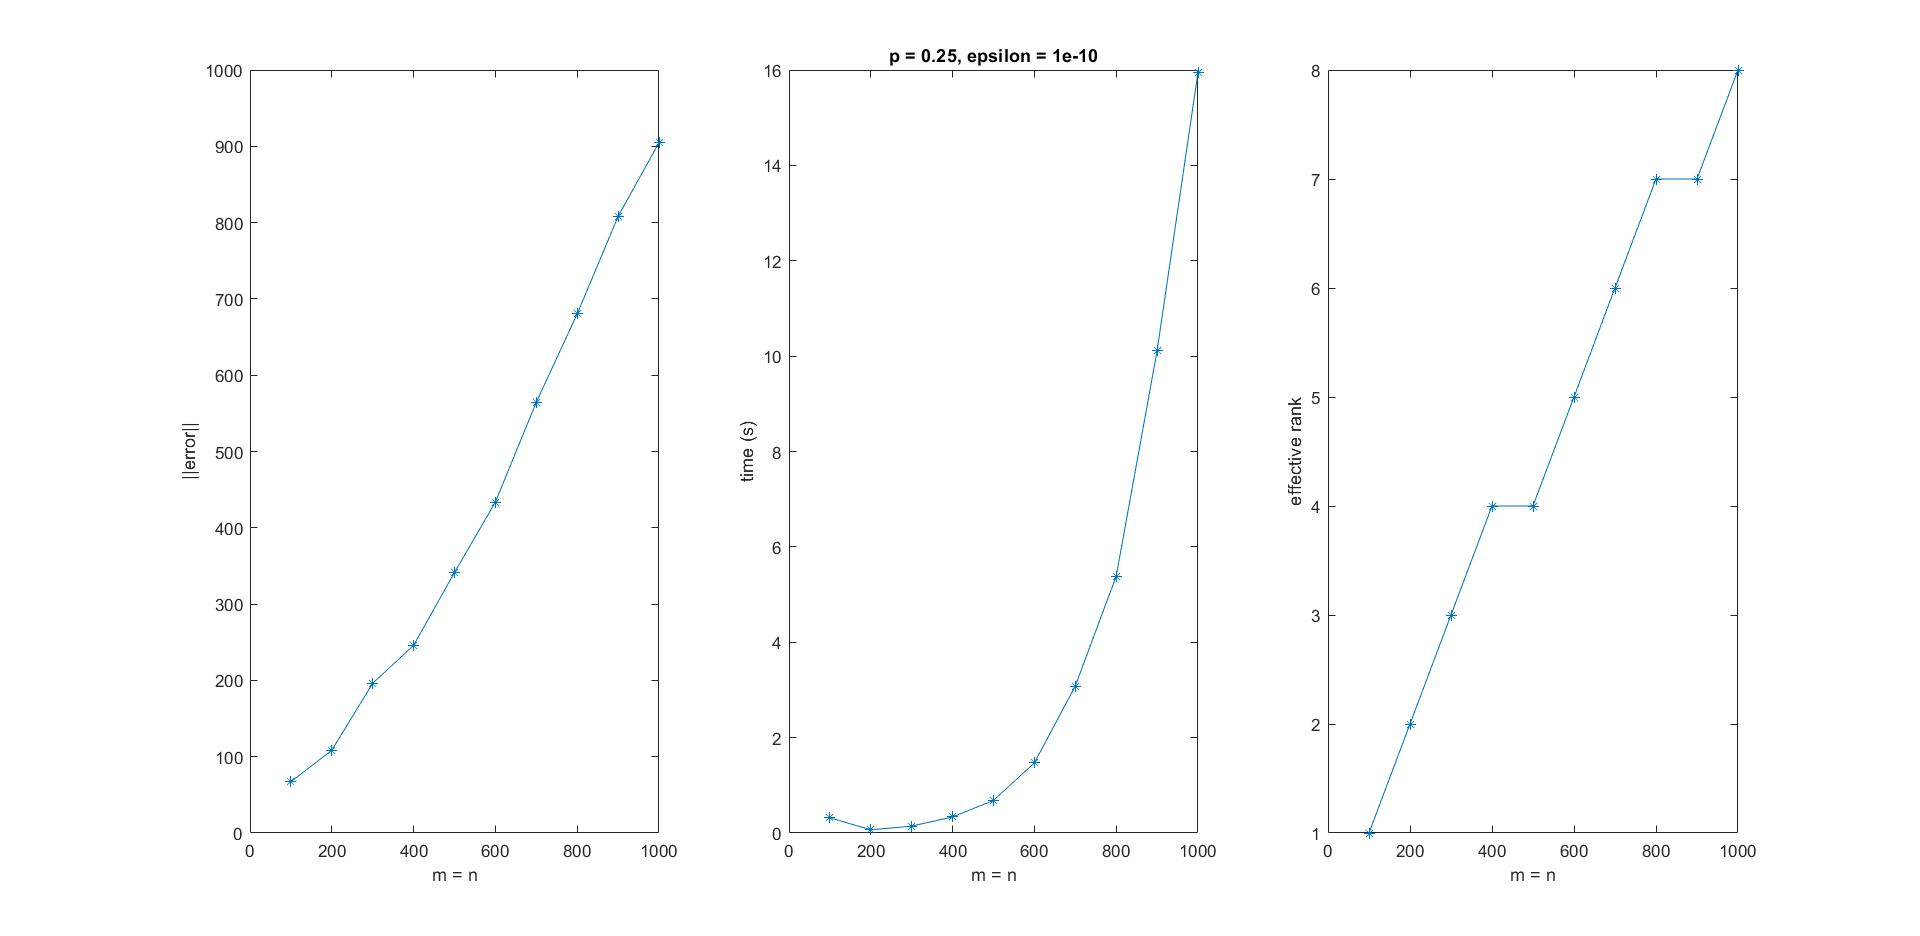
\includegraphics[width=\textwidth]{data/p1.jpg}
    \caption{$p = 0.25$, $\epsilon = 10^{-10}$}
    \label{img2}
\end{figure}
\begin{figure}[H]
    \centering
    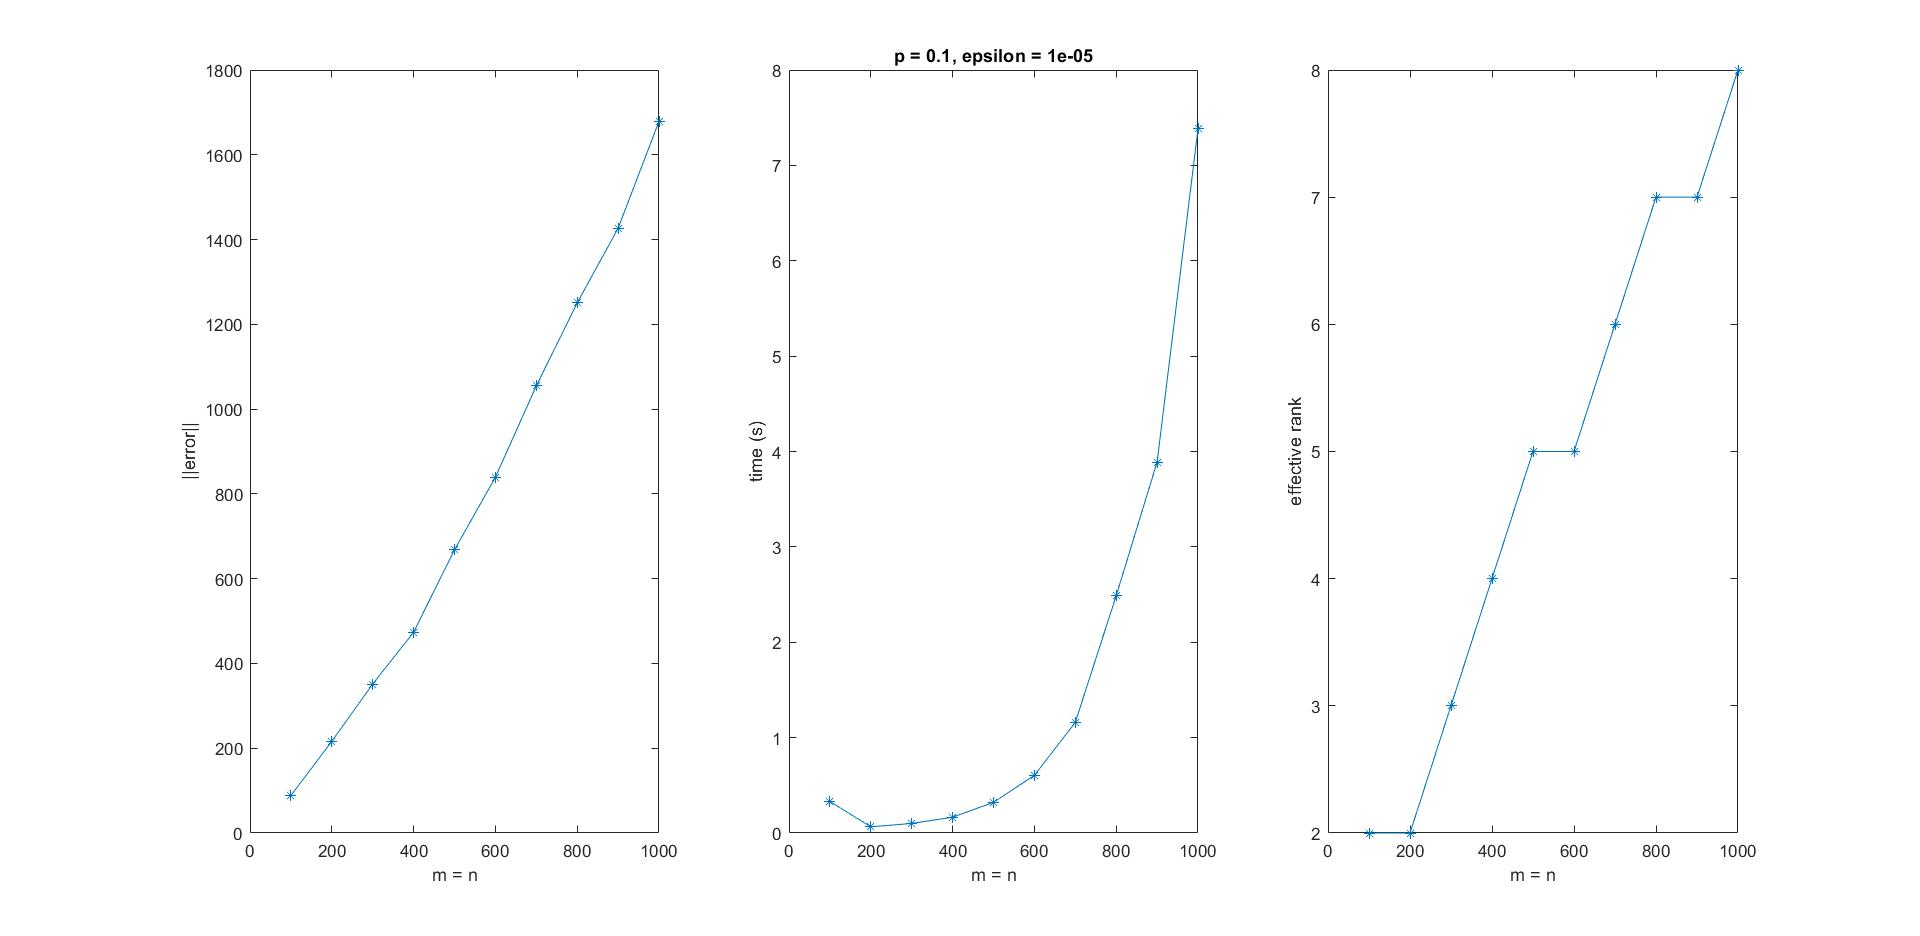
\includegraphics[width=\textwidth]{data/p3.jpg}
    \caption{$p = 0.1$, $\epsilon = 10^{-5}$}
    \label{img3}
\end{figure}
\begin{figure}[H]
    \centering
    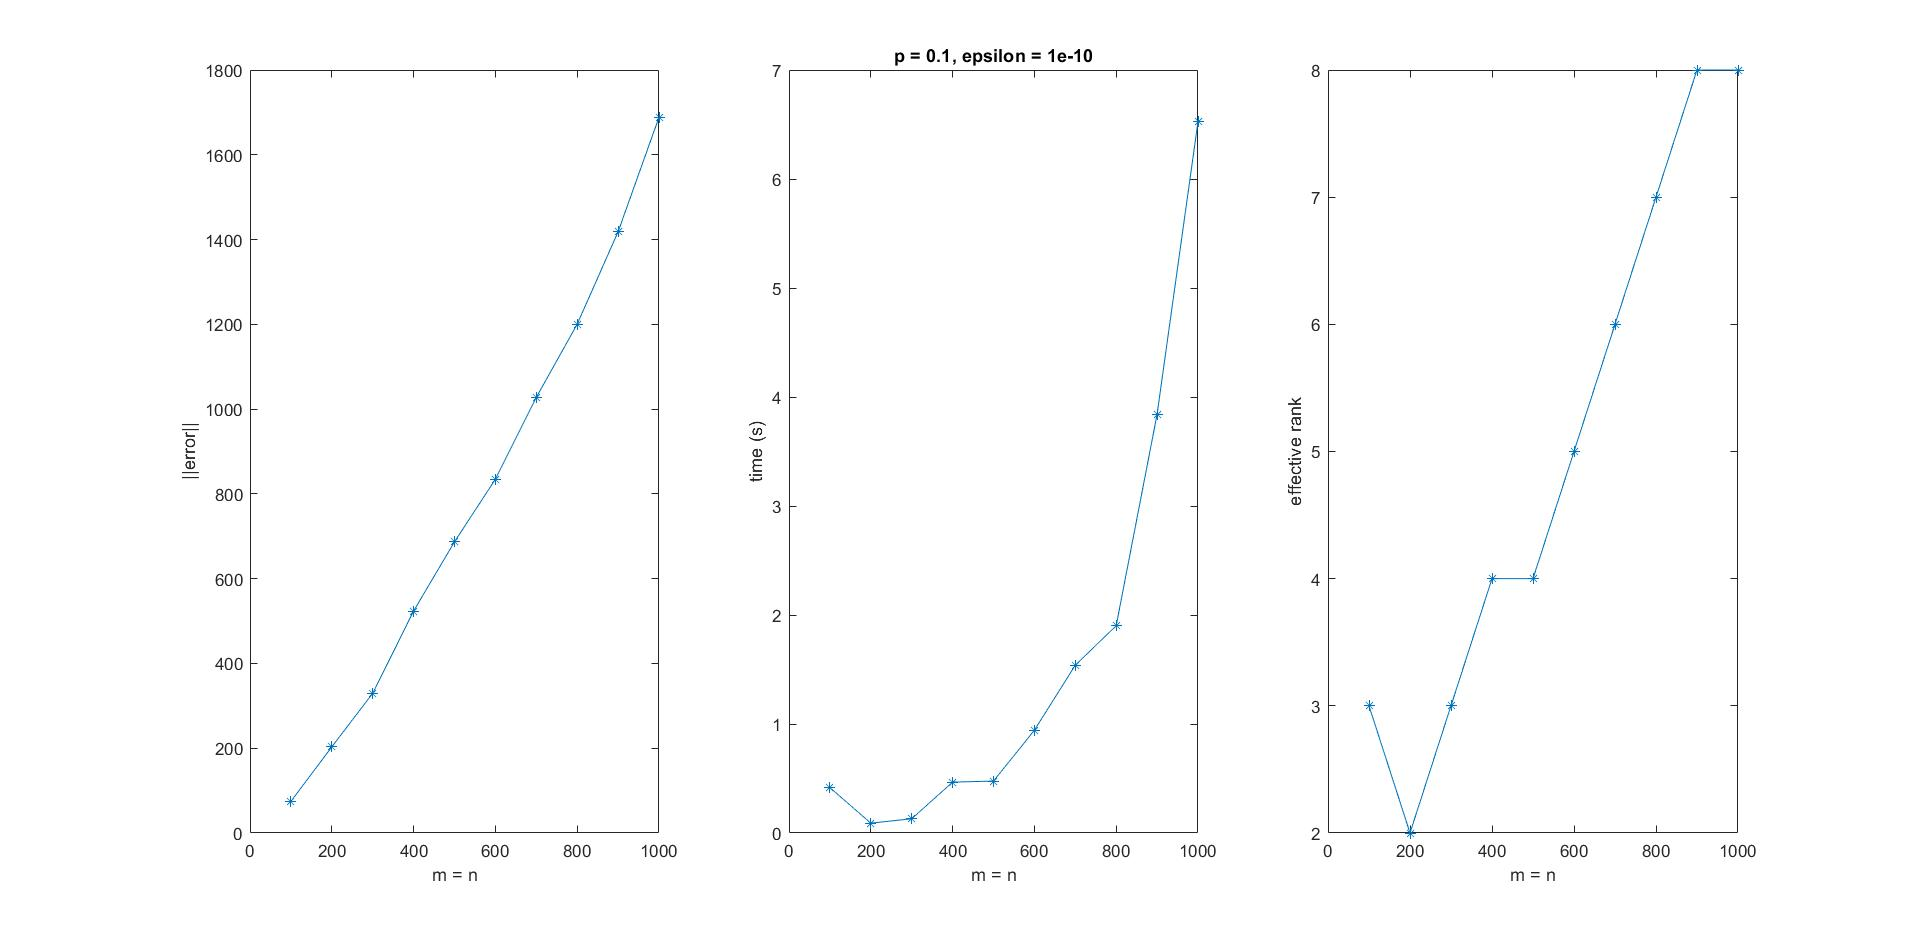
\includegraphics[width=\textwidth]{data/p2.jpg}
    \caption{$p = 0.1$, $\epsilon = 10^{-10}$}
    \label{img4}
\end{figure}


\begin{thebibliography}{}
\bibitem{FW} Frank, M., \& Wolfe, P. (1956). An algorithm for quadratic programming. Naval research logistics quarterly, 3(1-2), 95-110.

\bibitem{DH} Dunn, J. C., \& Harshbarger, S. (1978). Conditional gradient algorithms with open loop step size rules. Journal of Mathematical Analysis and Applications, 62(2), 432-444.

\bibitem{J} Jaggi, M. (2013). Revisiting Frank-Wolfe: Projection-free sparse convex optimization. In Proceedings of the 30th international conference on machine learning (No. CONF, pp. 427-435).

\bibitem{B} Boyd, S., Vandenberghe, L. (2004). Duality. In Convex Optimization (pp. 215-288). Cambridge: Cambridge University Press. doi:10.1017/CBO9780511804441.006


\bibitem{T} Tibshirani, R. (2015). \href{http://www.stat.cmu.edu/~ryantibs/convexopt-S15/lectures/23-cond-grad.pdf}{\textit{Conditional Gradient (Frank-Wolfe) Method}}, Carnegie Mellon University, PA.

\bibitem{FJSF} Fan, Z., Jeong, H., Sun, Y., \& Friedlander, M. P. (2020). Atomic Decomposition via Polar Alignment. \textit{Optimization}, 3(4), 280-366.

\end{thebibliography}

% --------------------------------------------------------------
%     You don't have to mess with anything below this line.
% --------------------------------------------------------------
 
\end{document}
